\begin{center}
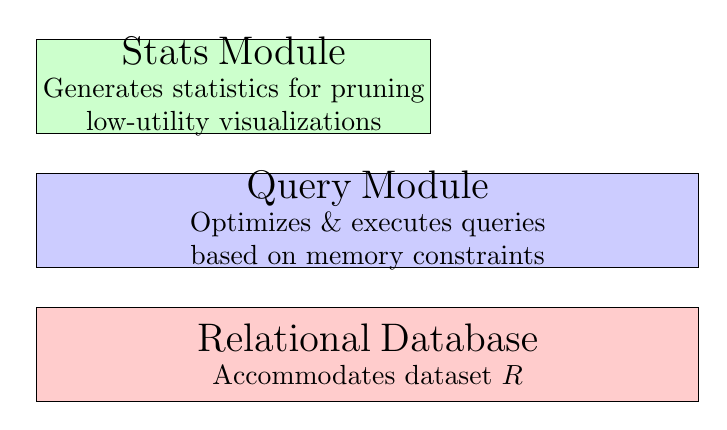
\begin{tikzpicture}
    \filldraw [fill={rgb:red,1;white,4}] (0, 0) rectangle (8.4, 1.2) node[pos=.5, align=center, text width=8cm] {{\Large Relational Database}\\ {\normalsize Accommodates dataset $R$}};
    \filldraw [fill={rgb:blue,1;white,4}] (0, 1.7) rectangle (8.4, 2.9) node[pos=.5, align=center, text width=8cm] {{\Large Query Module}\\ {\normalsize Optimizes \& executes queries based on memory constraints}};
    \filldraw [fill={rgb:green,1;white,4}] (0, 3.4) rectangle (5, 4.6) node[pos=.5, align=center, text width=5cm] {{\Large Stats Module}\\ {\normalsize Generates statistics for pruning low-utility visualizations}};
\end{tikzpicture}
\end{center}



\section{Algorithms \& Optimizations}
In this section, we describe the algorithms and optimizations to efficiently generate the hierarchy of recommended visualizations. To generate this hierarchy of visualizations, we explore the data subset lattice defined in Section 2, which we refer to as just \emph{lattice}. We start with the two phase approach where we first generate the lattice of visualizations, and then work towards identifying the maximum utility subgraph of size $k$. Then, we present our online decision-making algorithms to identify an approximate solution in a single phase. 

%We start with the offline case when we have unbounded time to generate the complete lattice of visualizations, and then work towards identifying the maximum utility sublattice of size $k$. Then, we propose our online decision-making algorithms to identify an approximate solution by generating only a small subset of the lattice.

\subsection{Two Phase Algorithms \& Optimizations}
Given user input $c$ for the number of maximum constraints to specify a data subset, we first generate the partial lattice of visualizations corresponding to all data subsets defined by $c$ or fewer constraints. Then, we identify the informative (best explaining) parent visualization for every visualization in the partial lattice except for root, and establish connections among these parent-child pairs to generate a directed acyclic graph (DAG). Further, we assign weight to each edge on this DAG based on the distance between the probability distributions corresponding to parent and child visualization. Finally, within the DAG, we seek a connected subgraph induced by $k$ vertices including root that has maximum total edge weight. 

\textbf{Lattice Generation.} In the naive implementation, each visualization is translated into view queries that get executed independently on the DBMS. However, for a particular user input, the queries evaluated by \system\ are very similar--- differ only in terms of the constraints used for specifying data subset. This presents opportunities to intelligently merge and batch queries, reducing the number of queries issued to the database and, in turn, minimizing the number of scans of the underlying data. Sharing computation in our setting is a special case of the general problem of multi-query optimization; we discuss the relationship in more detail in Section X. Specifically, we apply the following optimizations:

View queries with the same attribute(s) in WHERE clause can be rewritten as a single query by repositioning the WHERE clause attribute(s) in GROUP BY clause. Therefore, instead of executing separate queries for views $(X, A(Y), C_1(Z)), (X, A(Y), C_2(Z)), \ldots, \\(X, A(Y), C_n(Z))$, we execute a single query for combined view $(\{X, Z\}, Y, NULL)$. 

After applying our WHERE clause optimization, Hierarchia is left with a hierarchy of queries where queries with more grouping attributes cover the results of queries with fewer grouping attributes. Therefore, instead of executing separate queries for views $(\{X, Z_a\}, Y, NULL), (\{X, Z_b\}, Y, NULL)$, where $Z_a \subsetneqq Z_b$, we execute query for the view $(\{X, Z_b\}, Y, NULL)$ whenever possible. 

It is beneficial to execute queries with as many grouping attributes as possible, which cover the results of lower level queries in hierarchy. We claim (and verify in Section X) that grouping can benefit performance so long as memory utilization for grouping stays under a threshold. Memory utilization is, in turn, proportional to the number of distinct groups present in a query. If a set of attributes $Z_1, \ldots, Z_l$ are used for grouping, the upper bound on the number of distinct groups is given by $\prod_{i=1}^{l}\lvert Z_i\rvert$. Given a memory budget S, the challenge is now to determine the optimal grouping of attributes that each respect the memory budget. Formally, the problem is:



\textbf{PROBLEM 1 (OPTIMAL GROUPING).} \emph{Given memory budget $M$, a set of grouping attributes $Z = \{Z_1, \ldots, Z_n\}$, and an integer $c \le n$, divide the set of all $c$-combinations of $Z$, $Z^c$, into groups $Z^c_1, \ldots, Z^c_h$ (where $Z^c_i \subseteq Z^c$ and $U Z^c_i = Z^c$) such that if a query $Q$ groups the table by any $Z^c_i$, the memory utilization for $Q$ does not exceed $M$.}

Notice that when $c = 1$, the above problem is isomorphic to the NP-Hard bin-packing problem. If we let each attribute ($1$-combination) $Z_i \in Z^1$ correspond to an item in the bin-packing problem with weight $log(\lvert Z_i\rvert)$, and set the bin size to be $log(M)$, then packing items into bins is identical to finding groups $Z^1_1, \ldots, Z^1_h$, such that the estimated size of any query result is below $M$. We use the standard first-fit algorithm to find the optimal grouping of $k$-combinations.

\textbf{Subgraph Identification.} We are considering a special case (root inclusion) of the following problem: given a graph $G=(V,E)$, edge weights $w:E\rightarrow R$, and an integer $k\in\{1,\ldots,\lvert V\rvert\}$, find a subset $V^\prime \subseteq V $of $k$ vertices (i.e. $\lvert V^\prime\rvert = k$) such that the subgraph induced by $V^\prime$  is connected and has maximum total edge weight (i.e. $\sum_{e\in E\cap(V^\prime\times V^\prime)}w(e)$ is maximized). This is known as the maximum weight connected $k$-induced subgraph (\textsc{Mwcis}) problem and can be shown to be NP-complete by a reduction from the Clique problem. The \textsc{Mwcis} problem have been studied by \cite{ErnstAlthaus2009}, who proposed the use of a $k$-cardinality tree to solve the problem.

%The results from queries on the lower level can be used to compute the results for queries on the higher level 

\paragraph{Second phase algorithms.} Given a lattice, generated in the first phase, the goal is to find a connected sub-graph with maximal utility. It often might be the case where the lattice is very large due to a large number of attributes or attribute values. In such case finding an optimal solution can be computationally challenging. Thus, in this work we focus on devising heuristic algorithms. One class of algorithms that are appropriate to our case are the top-down traversal algorithms. The idea is that we traverse the lattice from the root down, adding gradually nodes to our solution. We are promised to get a feasible solution since we are starting with the node, and only add nodes whose informative parents are already in the solution. Formally, we maintain a list of nodes, denoted \textit{frontier}. Frontier nodes are nodes that are not in the current solution, but can be added to it since there informative parent is there. Thus in each iteration we add node to the solution, and update the frontier with its children nodes. A specific implementation would need to specify a scoring function to nodes in frontier that is used to pop out the next node in each iteration.
One can design a scoring function based on the trade-off between performance and complexity. In the most simple case, we can use the edge weights to score nodes in the frontier. That is, at each point we add a node with the highest interestingness value. We note that this is quite a greedy approach. Specifically, we might miss visualizations with high utility that are in deeper levels of the graph. Thus, another approach would be to extent the horizon for which we calculate a nodes utility. We denote such approach as a look-ahead approach. With a free parameter $n$, we would like to assign a score to each frontier node the corresponds to the expected utility of adding this node and $n-1$ more nodes who are its descendants. For example, we can run BFP for each node in frontier treating it as a root. 

Another approach is probabilistic..

Local improvements of a given solution..

\subsection{Single Phase Algorithms \& Optimizations}
Instead of generating the visualizations corresponding to all data subsets (defined by $c$ or fewer constraints), which is intractable, we instead aim to make it tractable, by incrementally generating only a subset of the visualizations and exploiting these visualizations to identify an approximate solution. We compute coarse statistics for unexplored visualizations from the already explored visualizations, and use these statistics to decide if generating the unexplored visualizations leads to an improved solution with higher utility.
%In particular, we focus on computing coarse approximations of unseen/unexplored visualizations in data subset lattice by combining known/explored visualizations in the dimension combination lattice.

\textbf{Coarse Statistics for Unexplored Visualizations.} We compute coarse statistics for unexplored visualizations from the explored visualizations using the following techniques:

\underline{Inclusion-Exclusion Principle:} Based on the inclusion-exclusion principle, we compute coarse upper and lower bounds for unexplored visualizations in the data subset lattice from the combination of explored visualizations in the dimension combination lattice. Note that, to apply the inclusion-exclusion principle and subsequently compute these coarse bounds, the aggregate function ($f$) involved in the data subset lattice needs either to be of counting type, e.g., {\tt SUM, COUNT, PERCENTAGE}, or computed directly from the counting functions, e.g., {\tt AVERAGE = SUM / COUNT}. We derive upper and lower bounds for an unexplored visualization obtained by combining two explored visualizations (with same y-dimension and filter) along x-dimension. Our derivation also generalizes to unexplored visualizations obtained by combining more than two explored visualizations.
%\begin{theorem}
%Given two visualizations $v_i (A_i \subset A, m_i \in M, f_i \in F_\Sigma, C_i \in \{(a, a_{val}) \mid a \in (A - A_i)\ \wedge\ a_{val} \in values(a)\})$ and $v_j (A_j \subset A, m_j \in M, f_j \in F_\Sigma, C_j \in \{(a, a_{val}) \mid a \in (A - A_j)\ \wedge\ a_{val} \in values(a)\})$, if $v_i$ and $v_j$ have same y-dimension ($m_i = m_j\ \wedge\ f_i = f_j$) and filter ($C_i = C_j$), then for visualization $v_x$ that combines the x-dimensions of $v_i$ and $v_j$ ($A_x = A_i \cup A_j$) with same y-dimension ($m_x = m_i = m_j\ \wedge\ f_x = f_i = f_j$) and filter ($C_x = C_i = C_j$), the following relationships hold for each visualization element/y-value $m_{x, (\alpha, \beta)} \in v_x$ that corresponds to the intersection of visualization elements $m_{i, \alpha} \in v_i$ and $m_{i, \beta} \in v_j$: $$min(m_{x, (\alpha, \beta)}) = max(m_{i, \alpha} + m_{j, \beta} - 1, 0)$$ $$max(m_{x, (\alpha, \beta)}) = min(m_{i, \alpha}, m_{j, \beta})$$.
%\end{theorem}
\newtheorem{theorem}{Theorem}
\begin{theorem}
Given two visualizations $V_i (X_i, Y, \sigma)$ and $V_j (X_j, Y, \sigma)$ with same y-dimension ($Y$) and filter ($\sigma$), if visualization $V_{ij} (X_{ij} = X_i \cup X_j, Y, \sigma)$ combines the x-dimensions of $V_i$ and $V_j$  maintaining same y-dimension and filter, then the following relationships hold for each visualization element $y_{x_i,x_j} {\in} V_{ij}$ that corresponds to the intersection of element $y_{x_{i}}{\in}V_{i}$ and $y_{x_{j}} {\in} V_{j}$: $$min(y_{x_i,x_j}) = max(y_{x_{i}} + y_{x_{j}} - C, 0)$$ $$max(y_{x_i,x_j}) = min(y_{x_{i}}, y_{x_{j}}),$$ where $C = \sum_{x \in X_i} y_x = \sum_{x \in X_j} y_x = \sum_{x \in X_{ij}} y_x$.
\end{theorem}

\begin{figure}[bht]
\label{example}
\centering
\includegraphics[scale=0.5]{figures/Figure-3.pdf}
\caption{Coarse Statistics Example}
\end{figure}

Consider the visualizations presented in Figure 4. The first visualization \textit{(\{Gender\}, Percentage(*), Country = US)} presents gender distribution within US population. The second visualization \textit{(\{Race\}, Percentage(*), Country = US)} presents race distribution within the same population. Now as per Theorem 2.1, we can derive upper and lower bounds for visualization \textit{(\{Gender, Race\}, Percentage(*), Country = US)} that presents gender-race combined distribution for the US population.

$$min(Y_{Male, Blue}) = max(Y_{Male}+Y_{Blue}-100, 0) = max(75+80-100, 0) = 55$$
$$max(Y_{Male, Blue}) = min(Y_{Male}, Y_{Blue}) = min(75, 80) = 75$$
%$$min(Y_{Gender = Female, Race = Blue}) = max(Y_{Gender = Female}+Y_{Race = Blue}-100, 0)$$ 
%$$max(Y_{Gender = Female, Race = Blue}) = min(Y_{Gender = Female}, Y_{Race = Blue})$$

\underline{Subset Property:} Based on the subset property, we compute coarse upper bounds for unexplored visualizations from the explored visualizations. Note that, similar to the inclusion-exclusion principle, to apply the subset property and subsequently compute these upper bounds, the aggregate function ($f$) involved in the data subset lattice needs either to be of counting type or computed directly from the counting functions. 
\begin{theorem}
Given two visualizations $V_i (X, Y, \sigma_i)$ and $V_j (X, Y, \sigma_j)$ with same x- and y-dimension, if visualization $V_{ij} (X, Y, \sigma_{ij} \supset \sigma_i, \sigma_j)$ has the same x- and y- dimensions and its filter covers that of $V_i$ and $V_j$, then the following relationships hold for each visualization element $y_x {\in} V_{ij}$ that corresponds to the subset of elements $y_x {\in} V_{i}$ and $y_x {\in} V_{j}$: $$max(y_x {\in} V_{ij}) = min(y_x {\in} V_{i}, y_x {\in} V_{j}).$$
\end{theorem}
\notes{We present an example of subset property.}

\textbf{Approximation of Utility.} After computing the coarse statistics for unexplored visualizations, we compute the uncertain distance between visualizations where one or more visualizations are bounded by these coarse statistics. Further, we compute the uncertain utility of visualizations based on these uncertain distances. 

\notes{We discuss the distance functions that can be used to compute the distance between uncertain probability distributions.}

\underline{Heuristics:} We propose a set of heuristics that can be used to approximate the utility of an unexplored visualizations. Though the heuristics do not provide any guarantees regarding the actual utility of unexplored visualizations, these heuristics are useful in absence of tight bounds. 

1. Diversity among parents/ancestors is a potent heuristic that can be used to anticipate the utility of an unexplored visualization. In absence of diversity among the parent/ancestor distributions, an unexplored visualization is less likely to deviate from the parent/ancestor distributions.

2. Entropy of parent/ancestor distribution is another potent heuristic that can be useful in predicting the utility of an unexplored visualization. In absence of entropy, an unexplored visualization is less likely to deviate from its parent/ancestor distribution.




